% Options for packages loaded elsewhere
\PassOptionsToPackage{unicode}{hyperref}
\PassOptionsToPackage{hyphens}{url}
%
\documentclass[
]{book}
\usepackage{amsmath,amssymb}
\usepackage{lmodern}
\usepackage{ifxetex,ifluatex}
\ifnum 0\ifxetex 1\fi\ifluatex 1\fi=0 % if pdftex
  \usepackage[T1]{fontenc}
  \usepackage[utf8]{inputenc}
  \usepackage{textcomp} % provide euro and other symbols
\else % if luatex or xetex
  \usepackage{unicode-math}
  \defaultfontfeatures{Scale=MatchLowercase}
  \defaultfontfeatures[\rmfamily]{Ligatures=TeX,Scale=1}
\fi
% Use upquote if available, for straight quotes in verbatim environments
\IfFileExists{upquote.sty}{\usepackage{upquote}}{}
\IfFileExists{microtype.sty}{% use microtype if available
  \usepackage[]{microtype}
  \UseMicrotypeSet[protrusion]{basicmath} % disable protrusion for tt fonts
}{}
\makeatletter
\@ifundefined{KOMAClassName}{% if non-KOMA class
  \IfFileExists{parskip.sty}{%
    \usepackage{parskip}
  }{% else
    \setlength{\parindent}{0pt}
    \setlength{\parskip}{6pt plus 2pt minus 1pt}}
}{% if KOMA class
  \KOMAoptions{parskip=half}}
\makeatother
\usepackage{xcolor}
\IfFileExists{xurl.sty}{\usepackage{xurl}}{} % add URL line breaks if available
\IfFileExists{bookmark.sty}{\usepackage{bookmark}}{\usepackage{hyperref}}
\hypersetup{
  pdftitle={Modeling in Education, and Social Sciences Using R},
  pdfauthor={William M. Murrah},
  hidelinks,
  pdfcreator={LaTeX via pandoc}}
\urlstyle{same} % disable monospaced font for URLs
\usepackage{color}
\usepackage{fancyvrb}
\newcommand{\VerbBar}{|}
\newcommand{\VERB}{\Verb[commandchars=\\\{\}]}
\DefineVerbatimEnvironment{Highlighting}{Verbatim}{commandchars=\\\{\}}
% Add ',fontsize=\small' for more characters per line
\usepackage{framed}
\definecolor{shadecolor}{RGB}{248,248,248}
\newenvironment{Shaded}{\begin{snugshade}}{\end{snugshade}}
\newcommand{\AlertTok}[1]{\textcolor[rgb]{0.94,0.16,0.16}{#1}}
\newcommand{\AnnotationTok}[1]{\textcolor[rgb]{0.56,0.35,0.01}{\textbf{\textit{#1}}}}
\newcommand{\AttributeTok}[1]{\textcolor[rgb]{0.77,0.63,0.00}{#1}}
\newcommand{\BaseNTok}[1]{\textcolor[rgb]{0.00,0.00,0.81}{#1}}
\newcommand{\BuiltInTok}[1]{#1}
\newcommand{\CharTok}[1]{\textcolor[rgb]{0.31,0.60,0.02}{#1}}
\newcommand{\CommentTok}[1]{\textcolor[rgb]{0.56,0.35,0.01}{\textit{#1}}}
\newcommand{\CommentVarTok}[1]{\textcolor[rgb]{0.56,0.35,0.01}{\textbf{\textit{#1}}}}
\newcommand{\ConstantTok}[1]{\textcolor[rgb]{0.00,0.00,0.00}{#1}}
\newcommand{\ControlFlowTok}[1]{\textcolor[rgb]{0.13,0.29,0.53}{\textbf{#1}}}
\newcommand{\DataTypeTok}[1]{\textcolor[rgb]{0.13,0.29,0.53}{#1}}
\newcommand{\DecValTok}[1]{\textcolor[rgb]{0.00,0.00,0.81}{#1}}
\newcommand{\DocumentationTok}[1]{\textcolor[rgb]{0.56,0.35,0.01}{\textbf{\textit{#1}}}}
\newcommand{\ErrorTok}[1]{\textcolor[rgb]{0.64,0.00,0.00}{\textbf{#1}}}
\newcommand{\ExtensionTok}[1]{#1}
\newcommand{\FloatTok}[1]{\textcolor[rgb]{0.00,0.00,0.81}{#1}}
\newcommand{\FunctionTok}[1]{\textcolor[rgb]{0.00,0.00,0.00}{#1}}
\newcommand{\ImportTok}[1]{#1}
\newcommand{\InformationTok}[1]{\textcolor[rgb]{0.56,0.35,0.01}{\textbf{\textit{#1}}}}
\newcommand{\KeywordTok}[1]{\textcolor[rgb]{0.13,0.29,0.53}{\textbf{#1}}}
\newcommand{\NormalTok}[1]{#1}
\newcommand{\OperatorTok}[1]{\textcolor[rgb]{0.81,0.36,0.00}{\textbf{#1}}}
\newcommand{\OtherTok}[1]{\textcolor[rgb]{0.56,0.35,0.01}{#1}}
\newcommand{\PreprocessorTok}[1]{\textcolor[rgb]{0.56,0.35,0.01}{\textit{#1}}}
\newcommand{\RegionMarkerTok}[1]{#1}
\newcommand{\SpecialCharTok}[1]{\textcolor[rgb]{0.00,0.00,0.00}{#1}}
\newcommand{\SpecialStringTok}[1]{\textcolor[rgb]{0.31,0.60,0.02}{#1}}
\newcommand{\StringTok}[1]{\textcolor[rgb]{0.31,0.60,0.02}{#1}}
\newcommand{\VariableTok}[1]{\textcolor[rgb]{0.00,0.00,0.00}{#1}}
\newcommand{\VerbatimStringTok}[1]{\textcolor[rgb]{0.31,0.60,0.02}{#1}}
\newcommand{\WarningTok}[1]{\textcolor[rgb]{0.56,0.35,0.01}{\textbf{\textit{#1}}}}
\usepackage{longtable,booktabs,array}
\usepackage{calc} % for calculating minipage widths
% Correct order of tables after \paragraph or \subparagraph
\usepackage{etoolbox}
\makeatletter
\patchcmd\longtable{\par}{\if@noskipsec\mbox{}\fi\par}{}{}
\makeatother
% Allow footnotes in longtable head/foot
\IfFileExists{footnotehyper.sty}{\usepackage{footnotehyper}}{\usepackage{footnote}}
\makesavenoteenv{longtable}
\usepackage{graphicx}
\makeatletter
\def\maxwidth{\ifdim\Gin@nat@width>\linewidth\linewidth\else\Gin@nat@width\fi}
\def\maxheight{\ifdim\Gin@nat@height>\textheight\textheight\else\Gin@nat@height\fi}
\makeatother
% Scale images if necessary, so that they will not overflow the page
% margins by default, and it is still possible to overwrite the defaults
% using explicit options in \includegraphics[width, height, ...]{}
\setkeys{Gin}{width=\maxwidth,height=\maxheight,keepaspectratio}
% Set default figure placement to htbp
\makeatletter
\def\fps@figure{htbp}
\makeatother
\setlength{\emergencystretch}{3em} % prevent overfull lines
\providecommand{\tightlist}{%
  \setlength{\itemsep}{0pt}\setlength{\parskip}{0pt}}
\setcounter{secnumdepth}{5}
\usepackage{booktabs}
\ifluatex
  \usepackage{selnolig}  % disable illegal ligatures
\fi
\usepackage[]{natbib}
\bibliographystyle{apalike}

\title{Modeling in Education, and Social Sciences Using R}
\author{William M. Murrah}
\date{2021-08-16}

\begin{document}
\maketitle

{
\setcounter{tocdepth}{1}
\tableofcontents
}
\hypertarget{preface}{%
\chapter*{Preface}\label{preface}}
\addcontentsline{toc}{chapter}{Preface}

\hypertarget{intro}{%
\chapter{Introduction to Simple Models}\label{intro}}

This chapter of the notebook corresponds to chapters 1 and 2 of \citet{judd2017data}.

\hypertarget{sampdist}{%
\chapter{Sampling Distributions and Statistical Inference}\label{sampdist}}

This chapter of the notebook corresponds to chapters 3 and 4 of \citet{judd2017data}.

\hypertarget{simple}{%
\chapter{Simple Regression}\label{simple}}

This chapter of the notebook corresponds to chapter 5 of \citet{judd2017data}.

\hypertarget{modeleval}{%
\chapter{Model Evaluation}\label{modeleval}}

This chapter of the notebook corresponds to Chapter 13 of \citet{judd2017data}.

\hypertarget{multiple}{%
\chapter{Models with Multiple Categorical Predictors}\label{multiple}}

This chapter of the notebook corresponds to chapter 6 of \citet{judd2017data}.

\hypertarget{Interaction}{%
\chapter{Moderation and Nonlinear Models}\label{Interaction}}

This chapter of the notebook corresponds to chapter 7 of \citet{judd2017data}.

\hypertarget{singlecat}{%
\chapter{Models with Single Categorical Predictor}\label{singlecat}}

This chapter of the notebook corresponds to chapter 8 of \citet{judd2017data}.

\hypertarget{multicat}{%
\chapter{Models with Multiple Categorical Predictors}\label{multicat}}

This chapter of the notebook corresponds to chapter 9 of \citet{judd2017data}.

\hypertarget{ancova}{%
\chapter{Models with Continuous and Categorical Predictors}\label{ancova}}

This chapter of the notebook corresponds to chapter 10 of \citet{judd2017data}.

\hypertarget{nonindependent}{%
\chapter{Models with Nonindependent Errors}\label{nonindependent}}

This chapter of the notebook corresponds to chapter 11 of \citet{judd2017data}.

\hypertarget{incorporating-predictors-with-nonindependent-data}{%
\chapter{Incorporating Predictors with Nonindependent Data}\label{incorporating-predictors-with-nonindependent-data}}

This chapter of the notebook corresponds to chapter 12 of \citet{judd2017data}.

\hypertarget{logistic-models-for-categorical-dependent-variables}{%
\chapter{Logistic Models for Categorical Dependent Variables}\label{logistic-models-for-categorical-dependent-variables}}

This chapter of the notebook corresponds to chapter 14 of \citet{judd2017data}.

\hypertarget{appendix-appendices}{%
\appendix}


\hypertarget{RSPL}{%
\chapter{Appendix A: R as a Statistical Programming Language}\label{RSPL}}

\hypertarget{overview}{%
\section{Overview}\label{overview}}

\begin{Shaded}
\begin{Highlighting}[]
\FunctionTok{library}\NormalTok{(knitr)}
\end{Highlighting}
\end{Shaded}

\begin{itemize}
\tightlist
\item
  Why use Statistical Programming Languages?
\end{itemize}

Computers and Programs

\begin{itemize}
\tightlist
\item
  Fixed program computer

  \begin{itemize}
  \tightlist
  \item
    programs are ``hard-wired'' into computer
  \item
    calculator, stopwatch
  \end{itemize}
\item
  Stored program computer

  \begin{itemize}
  \tightlist
  \item
    machine stores and executes instructions
  \item
    most modern computers, your phone, etc.
  \end{itemize}
\end{itemize}

Statistical Programs versus Statistical Programming Language

\begin{itemize}
\tightlist
\item
  Statistical Programs

  \begin{itemize}
  \tightlist
  \item
    fixed menus
  \item
    limited procedures (at least in the menus)
  \item
    leads to compartmentalizing models (e.g.~ANOVA, regression, GLM)
  \end{itemize}
\item
  Statistical Programming Languages (SPLs)

  \begin{itemize}
  \tightlist
  \item
    Turing complete: if you can create an algorithm you can program it
  \item
    Very flexible
  \item
    Integration of models: One model to rule them all!
  \end{itemize}
\end{itemize}

Everythin

\hypertarget{elements-of-statistical-programming}{%
\section{Elements of Statistical Programming}\label{elements-of-statistical-programming}}

\hypertarget{basic-elements-of-a-good-spl}{%
\subsection{Basic Elements of a Good SPL}\label{basic-elements-of-a-good-spl}}

\begin{enumerate}
\def\labelenumi{\arabic{enumi}.}
\tightlist
\item
  a rich set of \textbf{primitive expressions}
\item
  mechanisms for \textbf{combining expressions} into more complex expressions
\item
  means of \textbf{abstraction}, which allow for naming and manipulating compound objects
\end{enumerate}

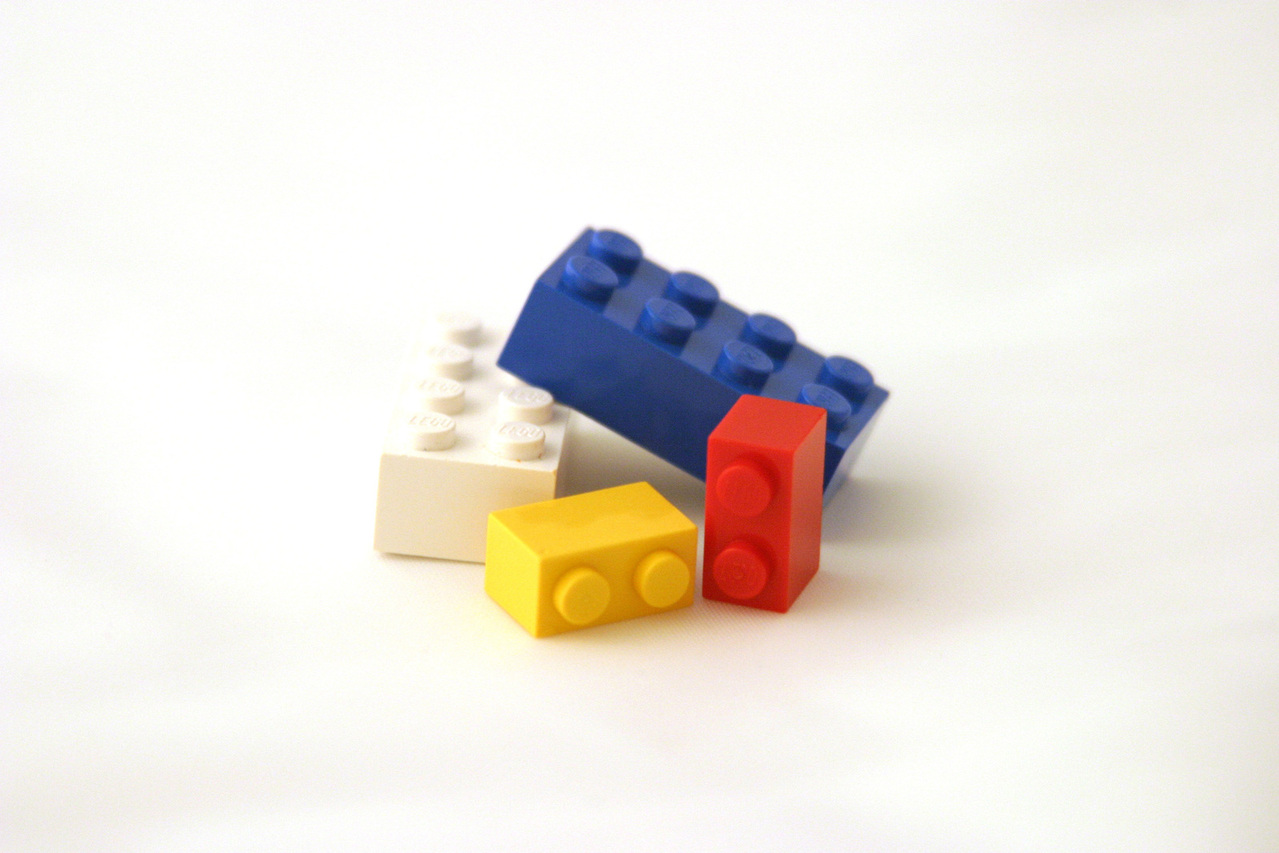
\includegraphics[width=0.4\linewidth]{figures/blocks}

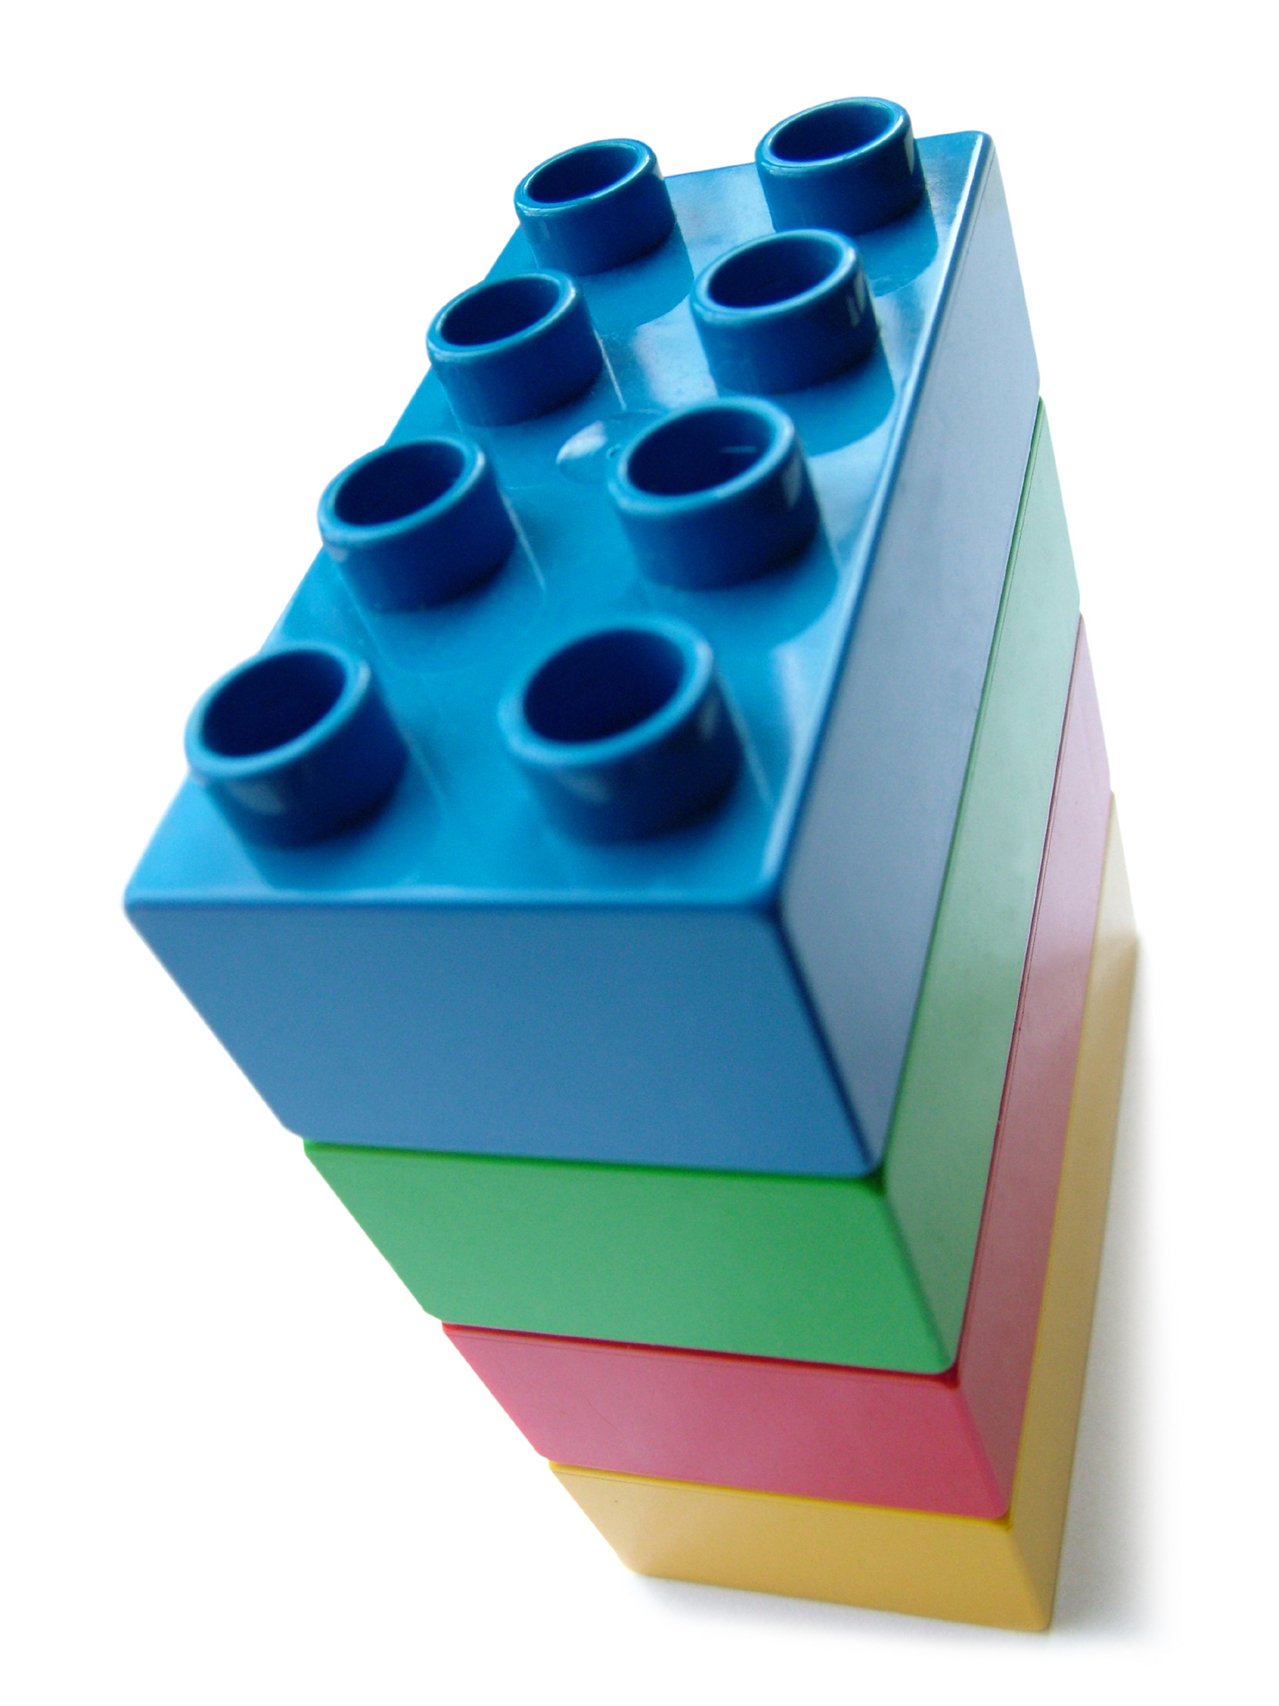
\includegraphics[width=0.2\linewidth]{figures/blockstack}

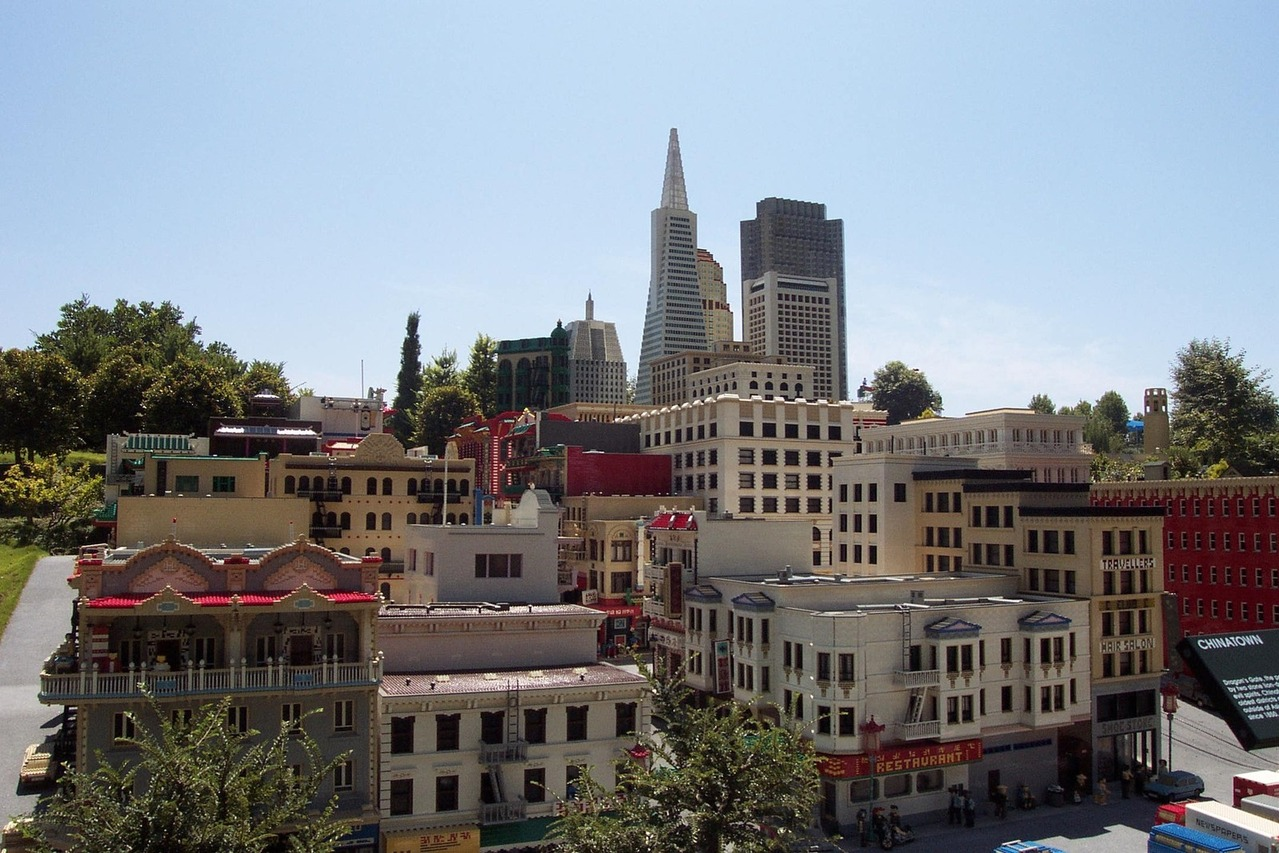
\includegraphics[width=0.4\linewidth]{figures/sanfran}

\hypertarget{expressions}{%
\section{Expressions}\label{expressions}}

\hypertarget{primitive-expressions}{%
\section{Primitive Expressions}\label{primitive-expressions}}

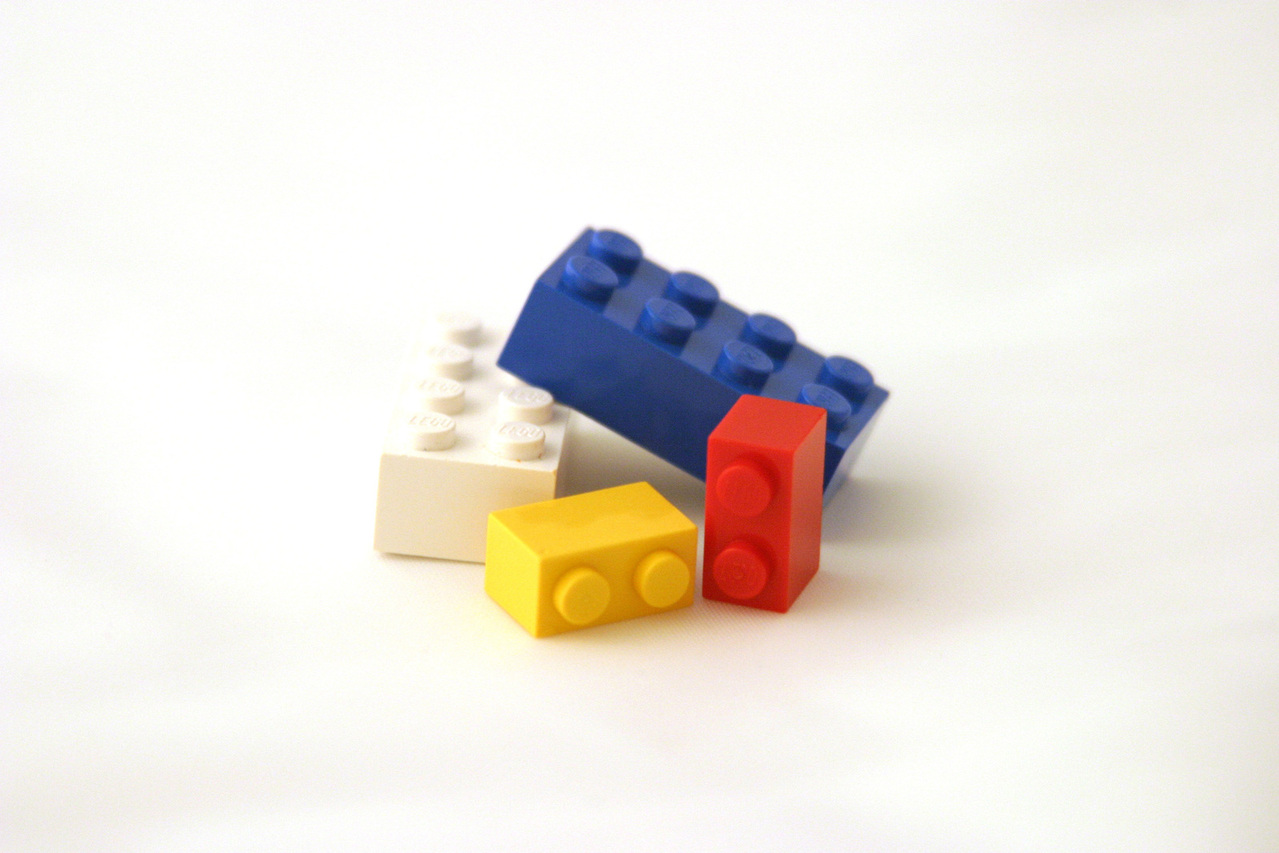
\includegraphics[width=0.3\linewidth]{figures/blocks}

\begin{itemize}
\item
  Everything in R is an object
\item
  Primitive objects are the simplest elements of a programming language, and include:

  \begin{itemize}
  \tightlist
  \item
    \emph{primitive data}
  \item
    \emph{primitive functions}
  \end{itemize}
\item
  They can be thought of as the basic building blocks for everything else in the language.
\item
  An \textbf{expression} is an input that the programming language can evaluate, and consists of function and data objects.
\end{itemize}

\hypertarget{primitive-data-types}{%
\section{Primitive Data Types:}\label{primitive-data-types}}

Data objects are the primary means of storing information in R.
R has a few basic \emph{data types}:

\begin{itemize}
\item
  \textbf{Numeric} -

  \begin{itemize}
  \tightlist
  \item
    \texttt{numeric}

    \begin{itemize}
    \tightlist
    \item
      \texttt{int} - integers (\texttt{1,2})
    \item
      \texttt{num} - real number (\texttt{1.2,\ -3.1,\ 200.0})
    \end{itemize}
  \end{itemize}
\item
  \textbf{character} or \textbf{string} -

  \begin{itemize}
  \tightlist
  \item
    \texttt{character}

    \begin{itemize}
    \tightlist
    \item
      \texttt{"Hello\ world!"}, \texttt{"Ten"}, \texttt{\textquotesingle{}Cat\textquotesingle{}}
    \item
      \texttt{"This\ is\ a\ sentence,\ which\ is\ a\ string"}
    \item
      \texttt{"10"} ( in single or double quotes, as long as they match)
    \end{itemize}
  \end{itemize}
\item
  \textbf{Boolean} or \textbf{Logical}

  \begin{itemize}
  \tightlist
  \item
    \texttt{logical}

    \begin{itemize}
    \tightlist
    \item
      \texttt{TRUE} or \texttt{FALSE} (use operators such as \emph{or}, \emph{and} and \emph{not}).
    \item
      They will evaluate to numbers where \texttt{FALSE} evaluates to zero, and \texttt{TRUE} evaluates to one.
    \item
      For example. if you enter \texttt{TRUE\ +\ 1} you will get \texttt{2} in return.
    \end{itemize}
  \end{itemize}
\end{itemize}

\begin{Shaded}
\begin{Highlighting}[]
\FunctionTok{mode}\NormalTok{(}\ConstantTok{TRUE}\NormalTok{)}
\end{Highlighting}
\end{Shaded}

\begin{verbatim}
## [1] "logical"
\end{verbatim}

\begin{Shaded}
\begin{Highlighting}[]
\ConstantTok{TRUE} \SpecialCharTok{+} \DecValTok{1}
\end{Highlighting}
\end{Shaded}

\begin{verbatim}
## [1] 2
\end{verbatim}

\hypertarget{primitive-functions}{%
\section{Primitive Functions}\label{primitive-functions}}

R uses functions to do all computations.

\hypertarget{operators}{%
\subsection{Operators}\label{operators}}

\begin{itemize}
\tightlist
\item
  Arithmetic Operators

  \begin{itemize}
  \tightlist
  \item
    +, -, *, /, \^{}
  \end{itemize}
\item
  Comparison (also called Boolean, Logical or Predicate) Operators

  \begin{itemize}
  \tightlist
  \item
    \texttt{\textless{},\ \textgreater{},\ ==,\ \textless{}=,\ \textgreater{}=,\ !=}
  \item
    less than, greater than, equal to, less than or equal to, greater than or equal to, not equal to
  \item
    return \texttt{TRUE} or \texttt{FALSE}
  \end{itemize}
\item
  Logical Operator

  \begin{itemize}
  \tightlist
  \item
    \texttt{\&}, \texttt{\textbar{}} ,\texttt{!}
  \item
    also return \texttt{TRUE} or \texttt{FALSE}
  \end{itemize}
\item
  Other functions

  \begin{itemize}
  \tightlist
  \item
    \texttt{mode()}
  \item
    \texttt{length()}
  \item
    \texttt{sum()}
  \item
    \texttt{sqrt()}
  \item
    \texttt{log()}
  \item
    \texttt{exp()}
  \end{itemize}
\item
  Assignment operators (assignment will be discussed below)

  \begin{itemize}
  \tightlist
  \item
    \texttt{\textless{}-} \textbf{preferred assignment operator - always use this one}
  \item
    \texttt{=} this will also work, but can be confusing (note different from \texttt{==}, the comparison operator)
  \item
    \texttt{-\textgreater{}} is also an assignment operator, but we will not use it.
  \end{itemize}
\end{itemize}

\hypertarget{programming-languages-are-not-forgiving}{%
\section{Programming Languages are Not Forgiving}\label{programming-languages-are-not-forgiving}}

\hypertarget{syntactically-valid-expressions}{%
\subsection{Syntactically valid expressions}\label{syntactically-valid-expressions}}

Expressions must be syntactically valid.

\begin{itemize}
\tightlist
\item
  syntax (form)

  \begin{itemize}
  \tightlist
  \item
    English: ``cat dog boy'' - not syntactically valid
  \item
    English: ``cat hugs boy'' - syntactically valid
  \end{itemize}
\item
  programming language:

  \begin{itemize}
  \tightlist
  \item
    ``hi'' 5 - not syntactically valid
  \item
    3.2*5 - syntactically valid
  \end{itemize}
\end{itemize}

\hypertarget{semantically-valid-expressions}{%
\subsection{Semantically valid expressions}\label{semantically-valid-expressions}}

\begin{itemize}
\tightlist
\item
  semantics - (meaning)

  \begin{itemize}
  \tightlist
  \item
    English: ``I are hungry'' - syntactically valid but semantic error
  \item
    programming language:

    \begin{itemize}
    \tightlist
    \item
      3 + ``hi'' - semantic error (you can't use addition on character strings)
    \end{itemize}
  \end{itemize}
\item
  Chomsky:
  ``colorless green ideas sleep furiously''
\end{itemize}

This statement is syntactically valid, but does not make sense, so makes a semantic error.

\hypertarget{assignment}{%
\section{Assignment}\label{assignment}}

We will often want to save data in a variable. We can do that with \textbf{assignment}, which utilizes an assignment operator.

\begin{Shaded}
\begin{Highlighting}[]
\NormalTok{x }\OtherTok{\textless{}{-}} \DecValTok{2}
\end{Highlighting}
\end{Shaded}

\begin{Shaded}
\begin{Highlighting}[]
\NormalTok{x}
\end{Highlighting}
\end{Shaded}

\begin{verbatim}
## [1] 2
\end{verbatim}

\begin{Shaded}
\begin{Highlighting}[]
\NormalTok{pet }\OtherTok{\textless{}{-}} \StringTok{"dog"}
\end{Highlighting}
\end{Shaded}

\begin{Shaded}
\begin{Highlighting}[]
\NormalTok{pet}
\end{Highlighting}
\end{Shaded}

\begin{verbatim}
## [1] "dog"
\end{verbatim}

\hypertarget{combining-expressions}{%
\section{Combining Expressions}\label{combining-expressions}}

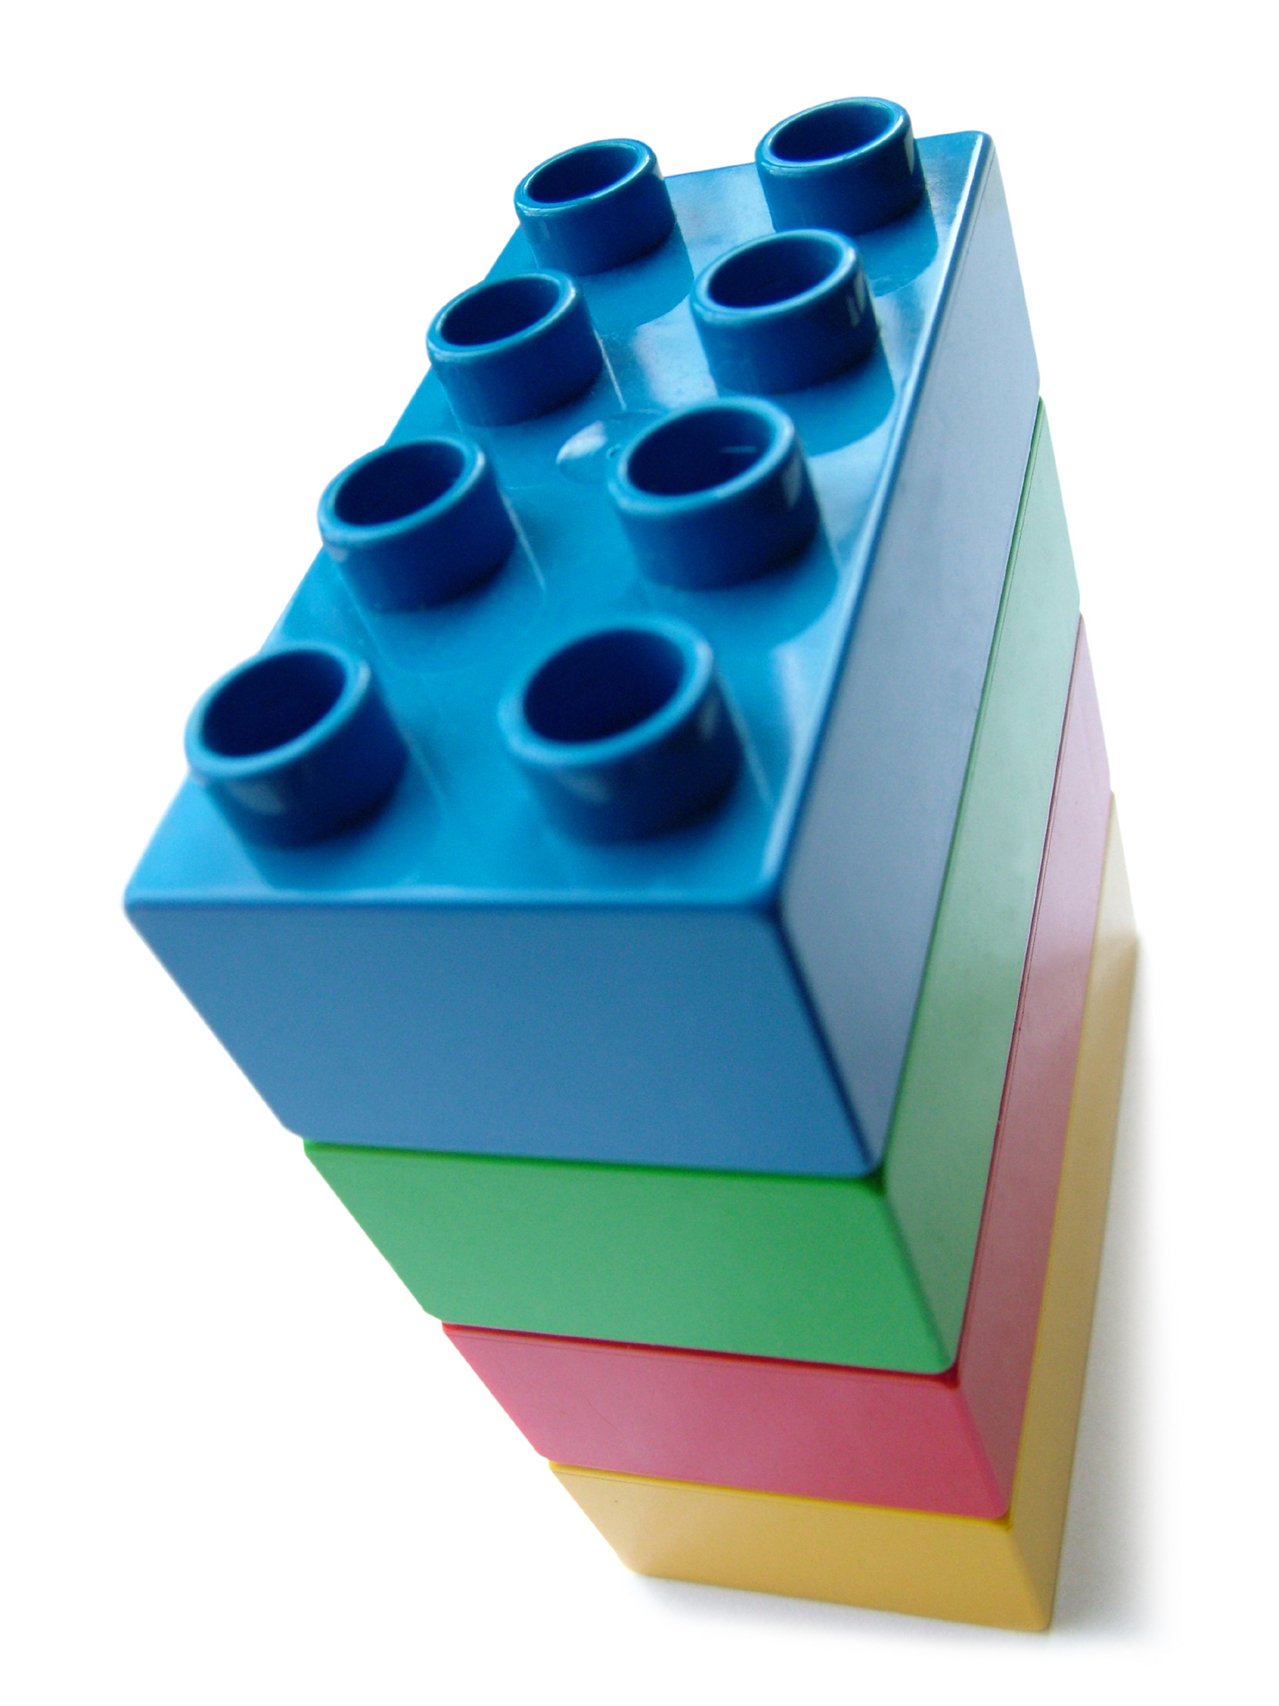
\includegraphics[width=0.3\linewidth]{figures/blockstack}

\hypertarget{complex-data-types}{%
\section{Complex Data Types}\label{complex-data-types}}

\begin{itemize}
\tightlist
\item
  Scalars, Vectors, Matrices, and Arrays
\item
  Lists
\item
  Dataframes
\end{itemize}

\hypertarget{grouping-homogeneous-data-types}{%
\section{Grouping Homogeneous Data Types}\label{grouping-homogeneous-data-types}}

\begin{itemize}
\tightlist
\item
  combining scalars
\end{itemize}

\begin{verbatim}
c()
\end{verbatim}

\begin{itemize}
\tightlist
\item
  combining expressions
\end{itemize}

\begin{verbatim}
{}
\end{verbatim}

\begin{itemize}
\tightlist
\item
  combining vectors
\end{itemize}

\begin{verbatim}
cbind()
rbind()
\end{verbatim}

\hypertarget{complex-functions}{%
\section{Complex Functions}\label{complex-functions}}

\begin{itemize}
\tightlist
\item
  Vectorization
\item
  Nested Functions
\item
  Loops and Conditional execution
\end{itemize}

class: inverse, center, middle

\hypertarget{abstraction}{%
\section{Abstraction}\label{abstraction}}

\hypertarget{abstraction-1}{%
\section{Abstraction}\label{abstraction-1}}

\begin{itemize}
\tightlist
\item
  Assignment
\item
\end{itemize}

\hypertarget{data-abstraction}{%
\section{Data Abstraction}\label{data-abstraction}}

\hypertarget{functional-abstraction}{%
\section{Functional Abstraction}\label{functional-abstraction}}

\hypertarget{anatomy-of-a-function}{%
\section{Anatomy of a Function}\label{anatomy-of-a-function}}

\begin{verbatim}
name <- function(arg_1, arg_2, ...) expression
\end{verbatim}

\hypertarget{teaching-with-a-statistical-programming-language}{%
\section{Teaching With A Statistical Programming Language}\label{teaching-with-a-statistical-programming-language}}

\hypertarget{an-example}{%
\subsection{An Example}\label{an-example}}

\hypertarget{mymean}{%
\section{myMean}\label{mymean}}

\hypertarget{basic-elements-of-a-good-spl-1}{%
\section{Basic Elements of a Good SPL}\label{basic-elements-of-a-good-spl-1}}

A rich set of \textbf{primitive expressions}

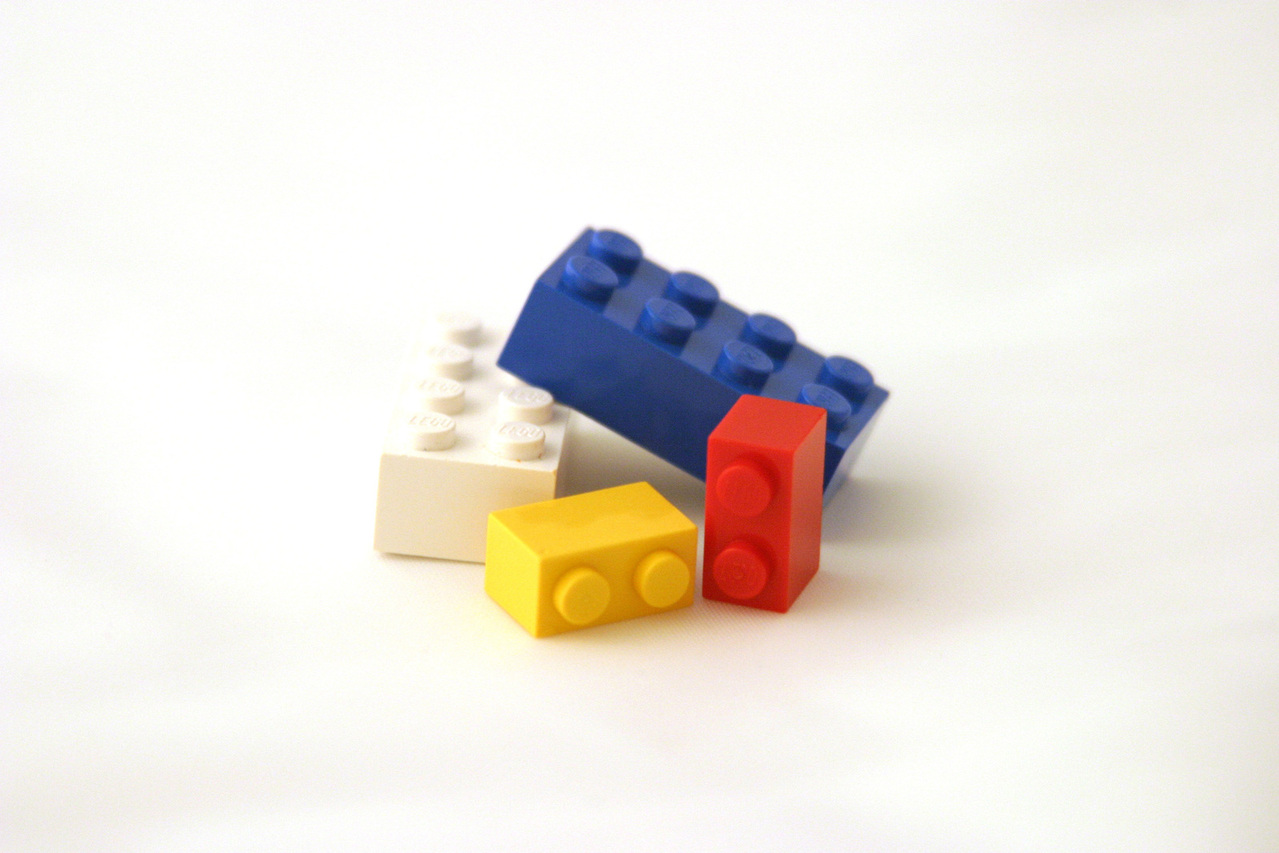
\includegraphics[width=0.3\linewidth]{figures/blocks}

Mechanisms for \textbf{combining expressions} into more complex expressions

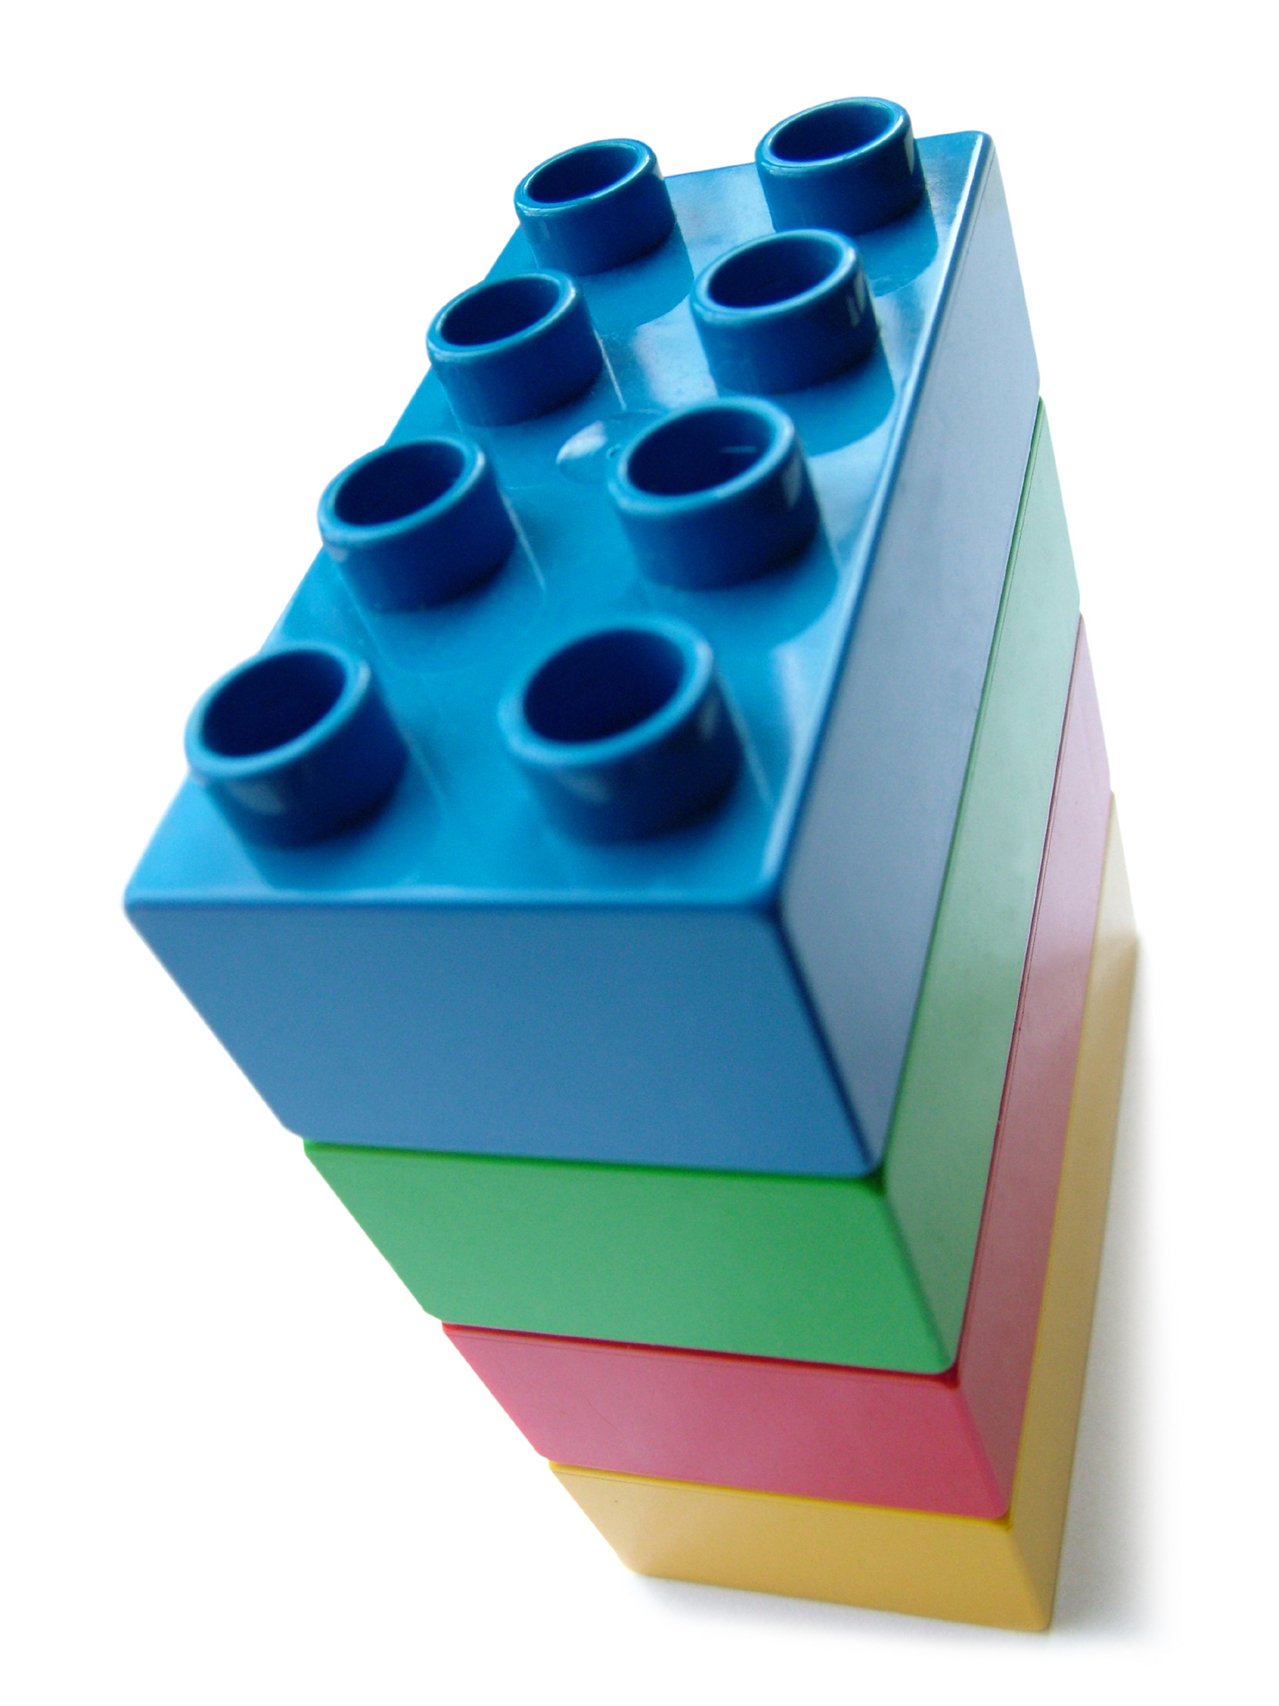
\includegraphics[width=0.1\linewidth]{figures/blockstack}

Means of \textbf{abstraction}, which allow for naming and manipulating compound objects

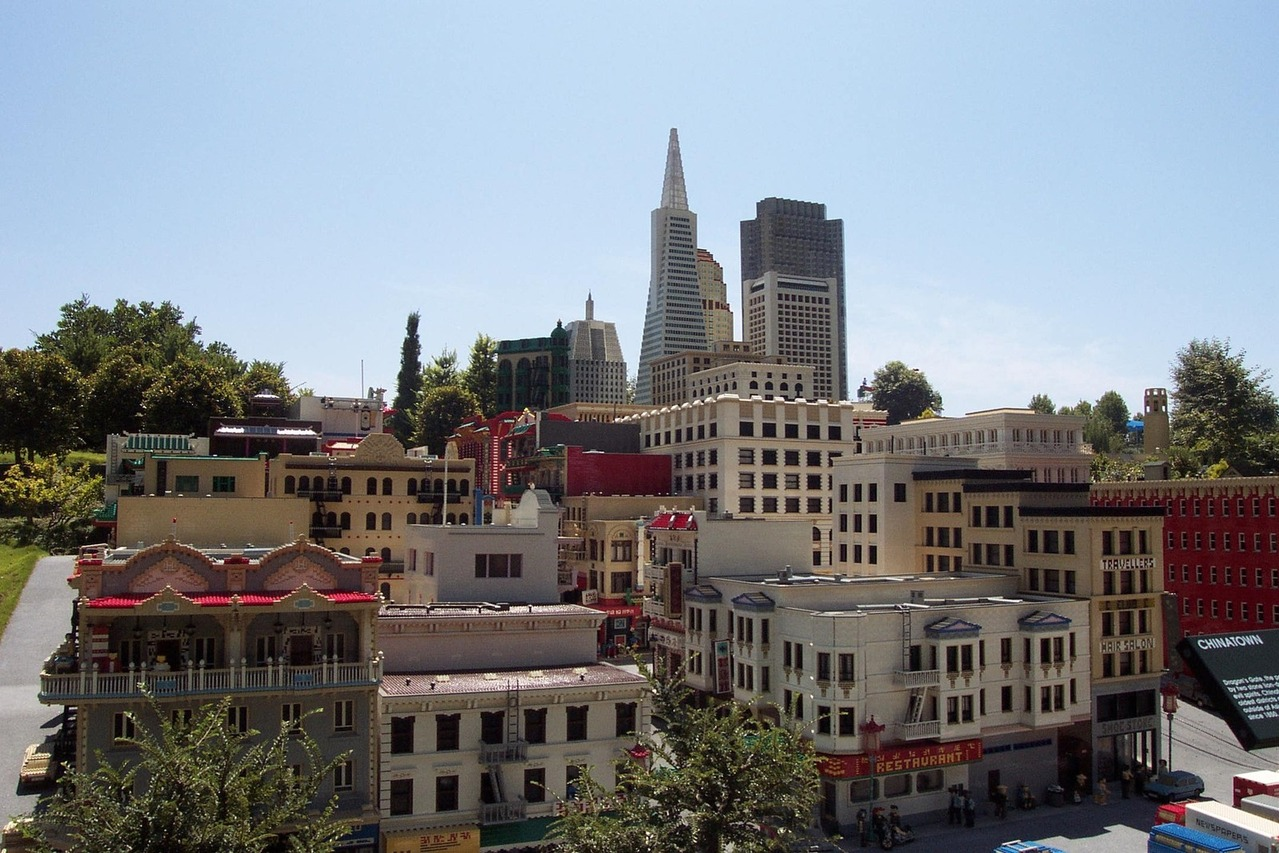
\includegraphics[width=0.4\linewidth]{figures/sanfran}

  \bibliography{book.bib,packages.bib}

\end{document}
